\documentclass[JCDReport.tex]{subfiles} 
\begin{document}

The VFS Browser is the GUI (Graphical User Interface) for the VFS Core.
With the browser it is possible to browse through existing or new file systems and perform the usual file system actions like delete, copy, move files or folders. Furthermore it serves as a client to the synchronization server which provides the user with the possibility to synchronize the file system with the a remote server.

\subsection{Requirements}
% TODO: Remove this text and replace it with actual content
% \emph{Describe which requirements (and possibly bonus requirements) you have implemented in this part.  Give a quick description (1-2 sentences) of each requirement. List the software elements (classes and or % functions) that are mainly involved in implementing each requirement.}

\subsubsection{Platform}
The browser is implemented as a desktop application and is written in C\# and uses WPF (Windows Presentation Foundation).\\
\textit{\textbf{Classes}: all classes in the VFSBrowser project}
% 1. The browser should be implemented on one of the following platforms: desktop, web or mobile.
% (a) Web applications written in C# must use Silverlight.
% (b) Web applications written in Java must either use Google Web Toolkit or JavaFX.
% (c) Mobile applications must target Android or Windows Phone.

\subsubsection{Operations}
The browser supports all operations of the VFS core.
\begin{itemize}
  \item Copy / Move / Rename / Delete
  \item Create folder
  \item Import / Export
  \item Create / Open / Close file system
\end{itemize}
\textit{\textbf{Classes}: MainViewModel\\
\textbf{Methods}: Copy, Move, Rename, Delete, NewFolder, ImportFile, ImportFolder, Export, OpenVfs, NewVfs, CloseVfs}
% 2. The browser should support all operations from Part 1 (VFS core). For example, users should be able to select a file/folder and copy it to another location without using console commands.

\subsubsection{Selection}
Selecting a file or a folder 
Multiple selection of files or folders is possible by pressing and holding down the Control- or Shift-Key and clicking with the left mouse button or with the Up- and Down-Key.\\
\textit{\textbf{Classes}: MainWindow.xaml\\
\textbf{View Items}: ItemsGrid}
% 3. The browser should support both single and multiple selection of files/folders.

\subsubsection{Keyboard navigation}
Most of the command are also executable by keyboard. All the other actions are accessible in the application menu, which can be opened by pressing the Alt-Key.\\
The keyboard commands in figure \ref{table:keyboardShortCuts} are available:\\
\textit{\textbf{Classes}: MainWindow.xaml\\
\textbf{View Items}: ItemsGrid}

\begin{figure}[h!]
	\centering
	\begin{tabular}{| l | l |}
		\hline
		\textbf{Command} & \textbf{Action} \\ \hline \hline
		Left / Back & Go to parent folder \\ \hline
		Right / Enter & Go to child folder / open file \\ \hline
		Up / Down & Select previous / next item \\ \hline
		Delete & Delete selected items \\ \hline
		F2 & Rename selected item \\ \hline
		Ctrl + C & Copy selected items \\ \hline
		Ctrl + X & Cut selected items \\ \hline
		Ctrl + V & Paste items \\ \hline	
	\end{tabular}
	\caption{Keyboard short cuts}
	\label{table:keyboardShortCuts}
\end{figure}

% 4. The browser should support keyboard navigation. The mandatory set of operations includes folder navigation, going to parent and child folders (this is optional for mobile applications due to limited keyboard functionality).

\subsubsection{Mouse navigation}
All the commands which are accessible by keyboard are also available with mouse navigation.
Most of them are found in the application menu or the context menu of the grid. Opening a folder or a file is achieved by double clicking the item with the left mouse button and to navigate to the parent folder, the folder ".." has to be double clicked. \\
\textit{\textbf{Classes}: MainWindow.xaml\\
\textbf{View Items}: ItemsGrid}
% 5. The browser should support mouse navigation (or touch in case of the mobile platform). The required operations are the same as in requirement 4.

\subsubsection{Search}	
The line beneath the application menu (see figure \ref{img:searchFunctions}) offers all the necessary tools to search for files or folder in the file system. In the drop down menu of the split button are the options listed in figure \ref{tbl:searchOptions} adjustable.\\
\textit{\textbf{Classes}: MainWindow.xaml, MainViewModel, \\
\textbf{Methods}: Search, CancelSearch}

\begin{figure}[h!]
	\centering
	\begin{tabular}{| l | p{10cm} |}
		\hline
		\textbf{Option} & \textbf{Description} \\ \hline \hline
		Case Sensitive & If checked, the search is case sensitive, otherwise insensitive. \\ \hline
		Global & If checked, the search is always started from the root folder, otherwise it is restricted to the current folder. \\ \hline
		Recursive & If checked, all results in the sub folders are also found, otherwise just the items in the current folder. \\ \hline
		\end{tabular}
	\caption{Search options}
	\label{tbl:searchOptions}
\end{figure}

\begin{figure}[h!]
  \centering
  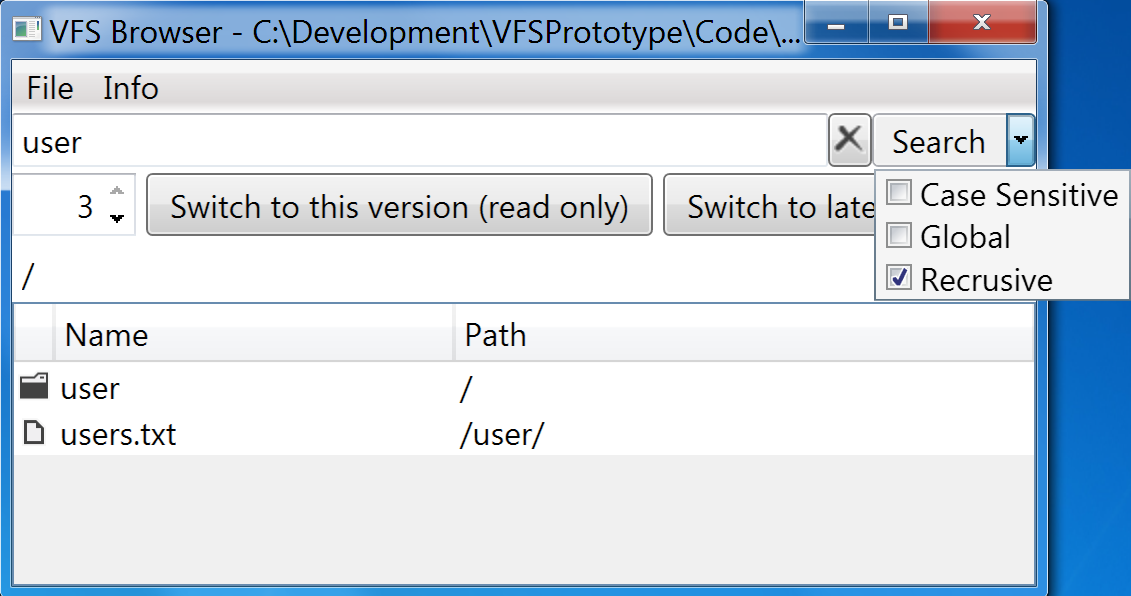
\includegraphics[scale=0.35]{Images/search.png} 
  \caption{Search functionality}
  \label{img:searchFunctions}
\end{figure}

% 6. The browser should support file-name search based on user-given keybwords. The search should provide options for: case sensitive/ case insensitive search; restrict search to folder; restrict search to folder and subfolders.	

\subsection{Bonus features}

\subsubsection{Responsive UI}
The VFS Browser includes a progress view (see figure \ref{img:progressView}), which is show during long-running operations (i.e import, copy). These operations can be cancelled by clicking the cancel button on the progress view.\\
\textit{\textbf{Classes}: OperationProgressView.xaml, OperationProgressViewModel, CopyCallbacks, ImportCallback, ExportCallbacks, CallbacksBase, FileSystemTextManipulator\\
\textbf{Methods}: Import, Export, Copy}

\begin{figure}[h!]
  \centering
  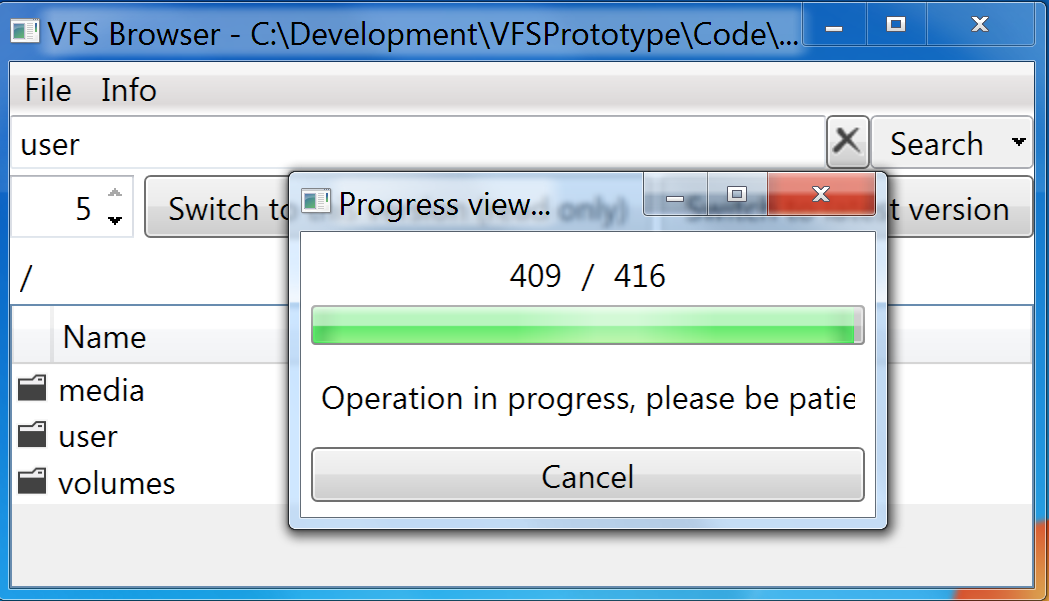
\includegraphics[scale=0.35]{Images/progress.png} 
  \caption{Progress view}
  \label{img:progressView}
\end{figure}
% 1. Responsive UI, i.e. the browser does not stall during long-running operations (i.e. file search or import). (3p)

\subsubsection{Advanced search}
Searching is implemented on a suffix basis. Therefore it is find files, by searching after a substring of the file name, in case you doesn't know the exact name.\\
\textit{\textbf{Classes}: SearchService \\
\textbf{Methods}: Search}
% 2. Advanced search; For example, search with wildcards/regexp, and approximate search based on some metric, e.g. edit distance. (2p)

\subsubsection{Operation progress}
The progress of long lasting operations like copying and importing is displayed in a separate window (see figure \ref{img:progressView}). The view shows the user the number of files involved in the operation and how many are already processed. This is displayed with text and also with a progress bar.\\
\textit{\textbf{Classes}: OperationProgressView.xaml, OperationProgressViewModel, CopyCallbacks, ImportCallback, ExportCallbacks, CallbacksBase, FileSystemTextManipulator\\
\textbf{Methods}: Import, Export, Copy}
% 3. Nice-to-have features like operation progress report (e.g. the number of files processed during export) or drag-and-drop for manipulative operations (move, copy, import). (2p)


\subsubsection{Drag-and-Drop}
Drag and Drop is implemented for importing files. It is possible to drag files and folders from the explorer into the grid in the VFSBrowser to copy them into the virtual file system.\\
\textit{\textbf{Classes}: MainWindow.xaml, MainViewModel, DropBehaviour \\
\textbf{Methods}: Drop}
% 3. Nice-to-have features like operation progress report (e.g. the number of files processed during export) or drag-and-drop for manipulative operations (move, copy, import). (2p)

\subsubsection{Efficient search}
The efficiency of the file search was improved, by building up a index with the file names. The index stores all file names and its suffixes and links them with the corresponding files. So it is possible to locate the files in O(n) time with n=keyword length.\\
\textit{\textbf{Classes}: IndexService, SuffixTree, SuffixTreeNode, SearchService, FileSystemTextManipulator\\
\textbf{Methods}: Search, AddToIndex, Index}
% 2. Effcient full-text search (using some sort of indexing). (4p)

\subsection{Design}
% TODO: Remove this text and replace it with actual content
% \emph{Give an overview of the design of this part and describe in general terms how the implementation works. You can mention design patterns used, class diagrams, definition of custom file formats, network protocols, or anything else that helps understand the implementation.}

\subsubsection{Design Patterns}
The GUI is implemented with the MVVM design pattern. The main advantages of this pattern is that the view is almost completely separated from the view model, except the data bindings. 
Events from the view are bound with commands in the view model, and therefore no code-behind is necessary. Furthermore manual UI test aren't needed, just the view model has to be tested, assuming that the binding to the view works.

\subsubsection{Search Index}
The search index is stored in a suffix tree. For each suffix of all file and folder names a sub tree is generated, and on each node the path to the file or folder is added. With that data structure it is possible to search for substring of file names in O(n) time, with n=length of keyword. 
The index is generated in a separate thread after opening a file system, and is kept uptodate after each modification. \\
\\
For example if the folder \textit{user} is added to the index, the tree in figure \ref{fig:searchIndex1} is build, and the path to the folder is added to each node.
After adding the folder \textit{usa} to the index, the tree would look like figure \ref{fig:searchIndex2}, and the path to the folder is added to the bold nodes.

\begin{figure}[h!]
  \centering
  \begin{minipage}{0.45\textwidth}
    \centering
    \Tree [. [.u [.s [.e r ] ] ] 
	    		 [.s [.e r ] ]
		    	 [.e r ]
		    	 [.r ]
		      ]
	\caption{Search index \textit{user}}
	\label{fig:searchIndex1}
  \end{minipage}
  \begin{minipage}{0.45\textwidth}
    \centering
    \Tree [. [.\textbf{u} [.\textbf{s} \textbf{a} [.e r ] ] ] 
	    		 [.\textbf{s} \textbf{a} [.e r ] ]
		    	 \textbf{a}
		    	 [.e r ]
		    	 [.r ]
		      ]
	\caption{Search index \textit{user, usa}}
	\label{fig:searchIndex2}
  \end{minipage}
\end{figure}

\subsection{Integration}
% TODO: Remove this text and replace it with actual content
% \emph{If you had to change the design or API of the previous part, describe the changes and the reasons for each change here.}

\subsubsection{Search Index}
For implementing the search index, the index service had to be integrated into the \textit{FileSystemTextManipulator}. So that after adding, copying or importing files, the file names of the new or changed files would be added to the index.


\end{document}
